\uuid{gKcH}
\exo7id{7635}
\auteur{mourougane}
\organisation{exo7}
\datecreate{2021-08-10}
\isIndication{false}
\isCorrection{true}
\chapitre{Autre}
\sousChapitre{Autre}

\contenu{
\texte{
On considère le contour $\Gamma$ et les points $w_1$, $w_2$, $w_3$ comme sur la figure ci-dessous
 \begin{center} 
 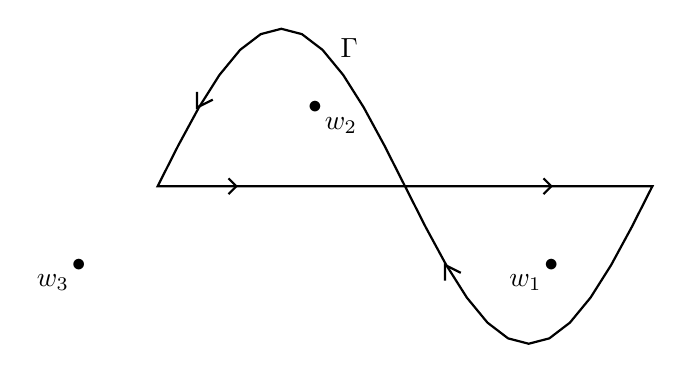
\begin{tikzpicture}
 %\draw [step=1cm, gray, very thin](-2,-4) grid (8,4);
 %\draw (-4,0) -- (4,0); \draw (0,-4) -- (0,4);
 \draw (5,-1) node {$\bullet$}; \draw (5,-1) node[below left] {$w_1$};
 \draw (2,1) node {$\bullet$};\draw (2,1) node [below right] {$w_2$};
 \draw (-1,-1) node {$\bullet$};\draw (-1,-1) node [below left] {$w_3$};
%\draw (1,0) node {$\bullet$}; \draw (1,0) node [below right] {$C$} circle (2) ;
\draw (2.2,2) node[below right] {${\Gamma}$};
%\draw [>=latex] (0,0) -- (1,1) arc (180:0:1) -- (4,0);
\draw[thick, draw=black](0,0) -- plot [domain=0:2*pi] (\x, {2*sin(\x r)}) -- cycle;
\draw [thick] (0.9,0.1)--(1,0)--(0.9,-0.1);
\draw [thick] (4.9,0.1)--(5,0)--(4.9,-0.1);
\draw [thick] (0.7,1.1)--(0.5,1)--(0.5,1.2);
\draw [thick] (3.85,-1.1)--(3.65,-1)--(3.65,-1.2);
\end{tikzpicture}
\end{center}
 Exprimer la valeur des intégrales suivantes à l'aide des nombres complexes $w_1,w_2,w_3$ :
}
\begin{enumerate}
    \item \question{$A=\int_\Gamma \frac{dz}{(z-w_1)(z-w_2)(z-w_3)}$.}
\reponse{On note d'abord que les indices de $w_1,w_2,w_3$ par rapport à $\Gamma$ sont respectivement $-1,1$ et $0$.
L'application $\Cc-\{w_1,w_2,w_3\}\to\Cc$, 
$z\mapsto \frac{1}{(z-w_1)(z-w_2)(z-w_3)}$ est méromorphe sur $\Cc$ avec des pôles simples en $w_1,w_2,w_3$ de résidu respectif 
$\lim_{z\to w_1}(z-w_1)\frac{1}{(z-w_1)(z-w_2)(z-w_3)}=\frac{1}{(w_1-w_2)(w_1-w_3)}$, $\frac{1}{(w_2-w_1)(w_2-w_3)}$, $\frac{1}{(w_3-w_1)(w_3-w_2)}$.
Par le théorème de Cauchy,
\begin{eqnarray*}
A&=&2i\pi\left(Ind_\Gamma(w_1)Res_{w_1}(f)+Ind_\Gamma(w_2)Res_{w_2}(f)+Ind_\Gamma(w_2)Res_{w_3}(f)\right)\\
&=&2i\pi\left(-\frac{1}{(w_1-w_2)(w_1-w_3)}+\frac{1}{(w_2-w_1)(w_2-w_3)}+0\right)\\
&=&\frac{2i\pi(w_1+w_2-2w_3)}{(w_2-w_1)(w_1-w_3)(w_2-w_3)}
\end{eqnarray*}}
    \item \question{$B=\int_\Gamma \sin(z)dz$.}
\reponse{L'application $\Cc\to\Cc$, 
$z\mapsto \sin z$ est holomorphe sur $\Cc$ étoilé : son intégrale sur le chemin fermé $\Gamma$ est donc nulle.}
    \item \question{$C=\int_\Gamma \frac{\sin(z) }{(z-w_1)^2}dz$.}
\reponse{Par le théorème de Cauchy pour les dérivées,
$$C=2i\pi Ind_\Gamma(w_1)\sin'(w_1)=-2i\pi\cos(w_1).$$}
\end{enumerate}
}
